There is plenty of literature available for the design and implementation of Graphics engines. None of the literature we have reviewed had information on the design of the API. It is much more likely to find generic information about programming\cite{Finney:2004:GPO:983901}, object-oriented development\cite{Eberly:2006:GED:1214590}, dynamic linking\cite{Zerbst:2004:GEP:983612} and coding guidelines\cite{Eberly:2004:GEA:1214185}.

In order to discuss the API of graphics engines, we will first have to look at the components of a graphics engine. There are many aspects of a graphics engine that need to be addressed when developing such a library. A very good overview to this subject is provided by \cite{bauchinger-2007-mre}. As our focus is on the API of the introductory articles, we will merely cover the API required by those tutorials.

The very first applications built when learning graphics development involve the programmatic generation of a scene. The developer usually learns these few operations at first:

\begin{smalllist}
	\item Placing objects in a 3d space,
	\item moving/rotating those objects to other positions,
	\item moving/rotating the camera to view the scene from different angles, and
	\item performing the repositioning operations discretely within a time frame.
\end{smalllist}

\section{Scene graph}

	 This data structure has become the de-facto standard for storing objects in graphics engines. Paffenroth et al. \cite{Paffenroth:2002:DSG:787261.787772} describe it as a ``well-known and longstanding notion in computer graphics, either as a structural hierarchy of the view scene \cite{Clay:1996:PLI:1435699.1437354}, or a spatial development of it \cite{Subramanian:1997:CDI:614267.614379}\cite{Sudarsky:1999:DSO:614273.614419}.''

	A \termdef{Scene Graph} usually is a direct acyclic graph containing objects in the scene\cite{Strauss:1992:OGT:142920.134089}. Each node within the tree has several properties (like location, orientation and scale) that usually propagate to child nodes. Placing a dinner table in a room could look as depicted in Figure \ref{fig:ExampleSceneGraph}. The objects ``on'' the table have a relative position referencing the position of the parent node. This solution allows us to reposition the complete structure without having to reposition each sub-node separately.

	\begin{figure}[htbp]
		\centering
		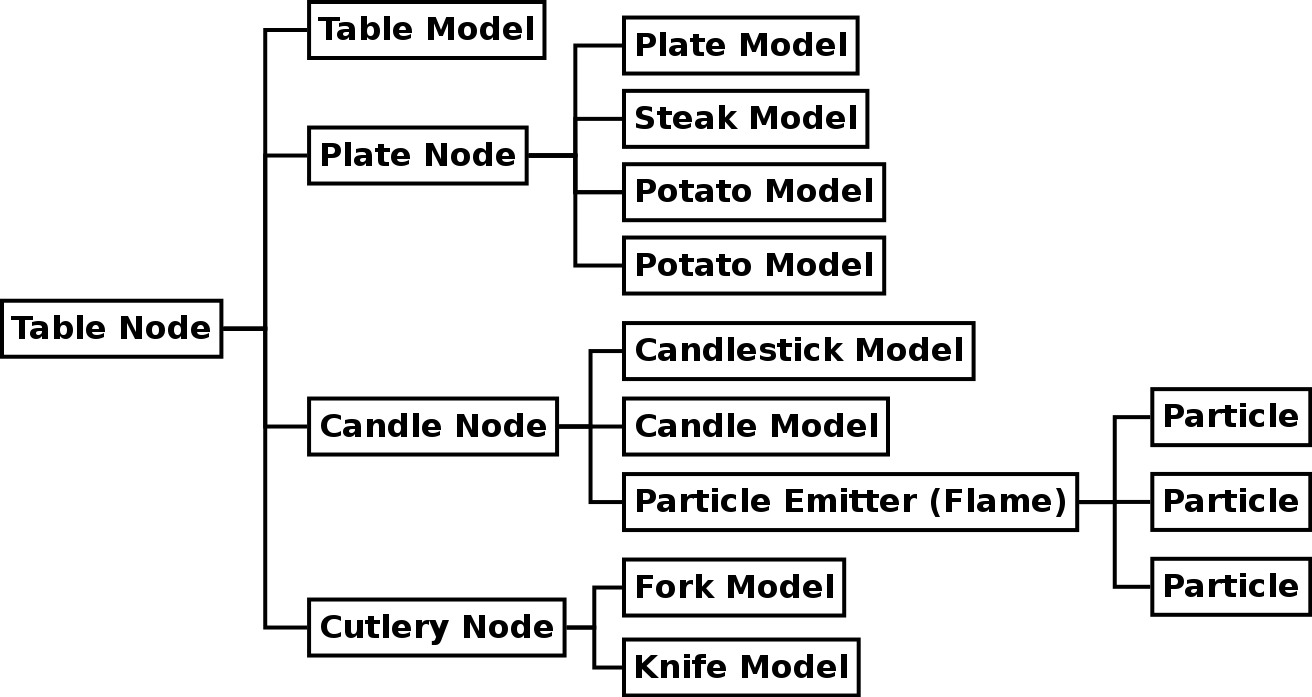
\includegraphics[width=14cm]{images/example-scenegraph.png}
		\caption{An example scene graph depicting a dinner table}
		\label{fig:ExampleSceneGraph}
	\end{figure}

	Apart from these usability features, scene graphs are further useful for the calculation of bounding volumes, which in turn are used for clipping. Assarson et. al summarize several such techniques and shows a speed improvement of up to 11-fold using these methods\cite{Assarsson:2000:OVF:360529.360537}.

\section{Quaternions}

	Positioning an object within a scene graph requires the expression of its orientation relative to its parent node. There are several methods for expressing the attitude of an object within 3-dimensional space, which are summarized in \cite{Diebel06}. The \termdef{quaternion} has become the de-facto standard for this purpose in graphics engines\cite{Mukundan02}, as it is neither as memory-intensive as a transformation matrix, nor prone to the so-called gimbal lock as Euler angles are.

	Quaternions are hyper-complex numbers of rank 4, constituting a four dimensional vector space over the field of real numbers\cite{birkhoff1960survey}. A Quaternion is expressed as a four tuple
	\[q = (w, x, y, z) = w + ix + jy + kz\]
	which consists of a vector part $x, y, z$, the scalar part $w$ and where the units $i$, $j$, $k$ satisfy:
	\begin{gather}
		i^{2} = j^{2} = k^{2} = ijk = -1 \\
		ij = -ji = k \\
		jk = -kj = i \\
		ki = -ik = j
	\end{gather}

	A quaternion expresses an attitude within 3d-space -- more precisely the rotation towards an attitude. The multiplication of quaternions ($A \cdot B$) correspond to sequential application of their rotations and yields a new quaternion ($C$) which expresses the first rotation followed by the second rotation. As the first rotation will rotate the axes of the second rotation, changing the order of the multiplicants results in a different compound rotation, rendering the quaternion multiplication non-commutative. This property of rotations is visualized in Figure \ref{fig:Rotations}.

	\begin{figure}[htbp]
		\centering
		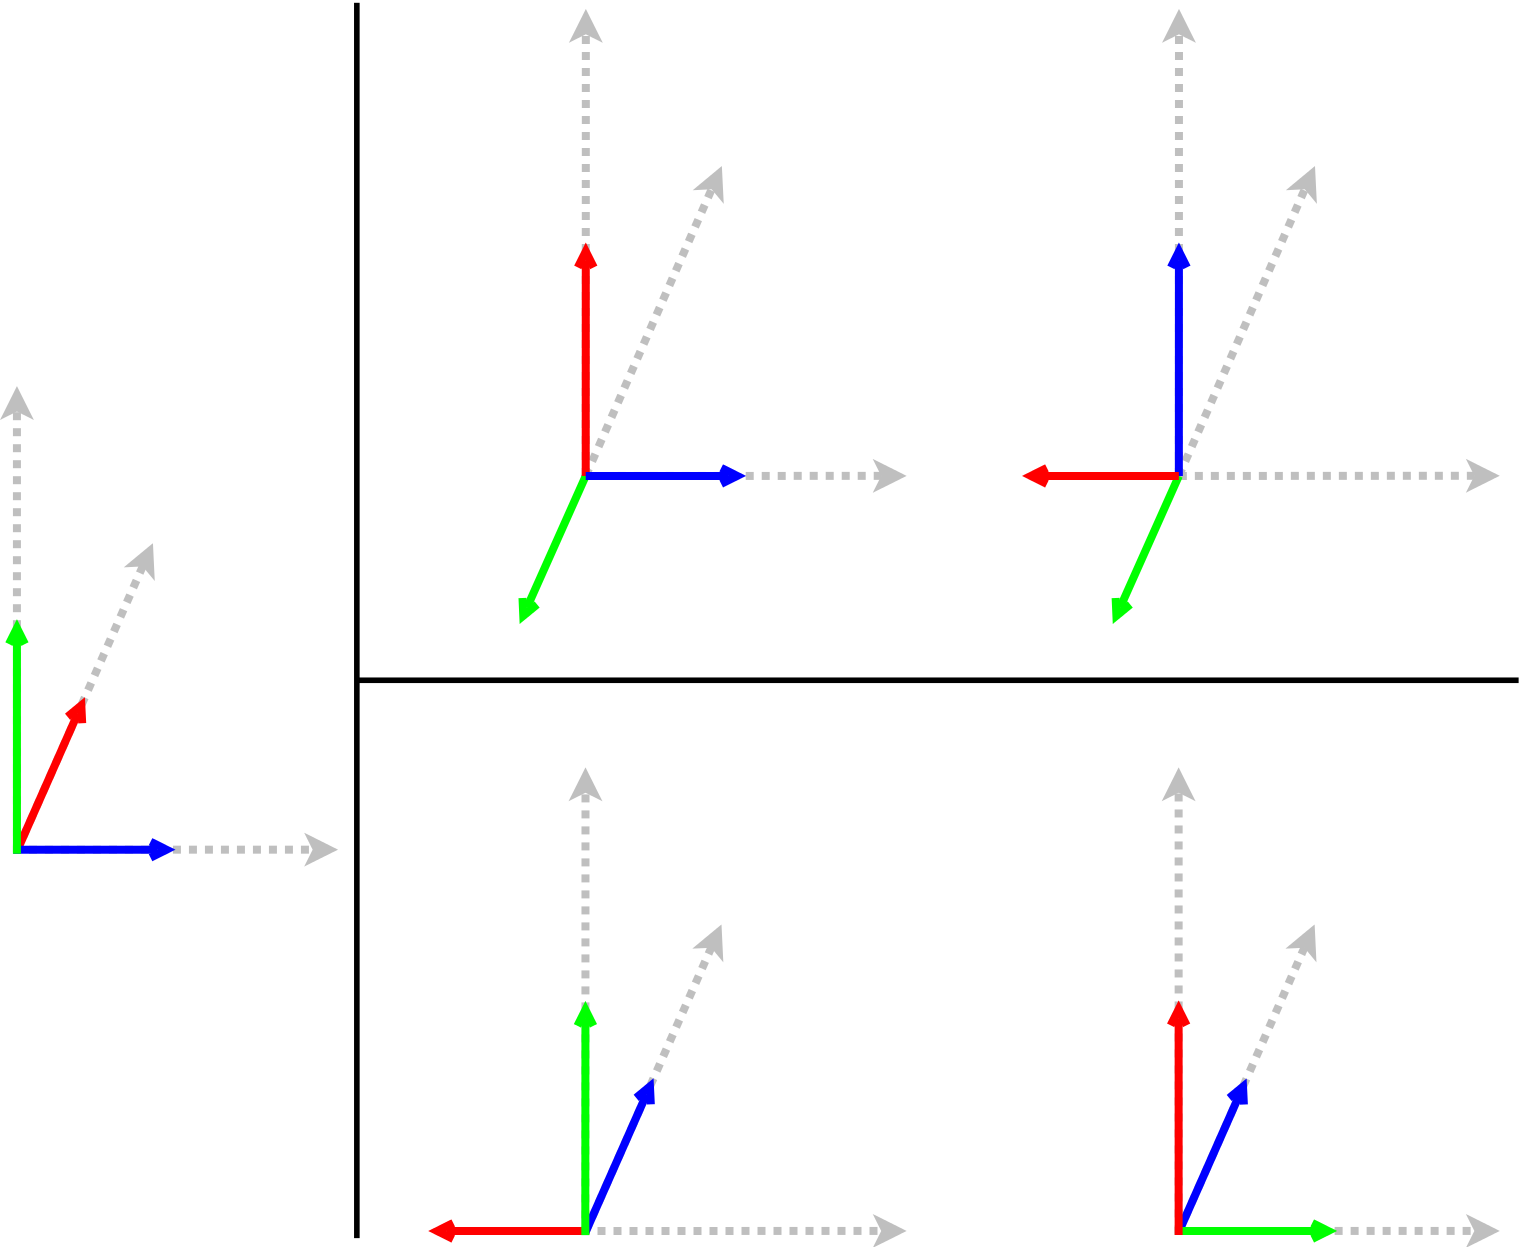
\includegraphics[width=14cm]{images/rotation.png}
		\caption{Changing the order of rotations yields different results: The rotations above (90\degree around blue, 90\degree around green) are applied to the original orientation in reverse order in the lower half, resulting in different final attitudes.}
		\label{fig:Rotations}
	\end{figure}

\section{Render Loop}

	\clubpenalty=10000
	\widowpenalty=10000
	Once the initial setup of a scene is completed, it needs to be drawn onto the screen each time an object in the scene is modified. Instead of rendering the output each time the scene is updated, most graphics engines choose to redraw it in an infinite loop, assuming that the output will change frequently enough that a constant redraw is necessary. This behavior is in contrast to that of window managers for example, which usually redraw the screen only when necessary.
	\clubpenalty=150
	\widowpenalty=150

	There are several aspects to the design of this infinite loop. Valente et al.\ \cite{Valente_Conci_Feijo_2005} list and categorize several such models. The most simple implementation, the ``simple coupled model'', is visualized in Figure \ref{fig:RenderLoopSimple}. The objects are updated with fixed values in this model -- the camera rotates 1\degree each frame, for example.

	\begin{figure}[htbp]
		\centering
		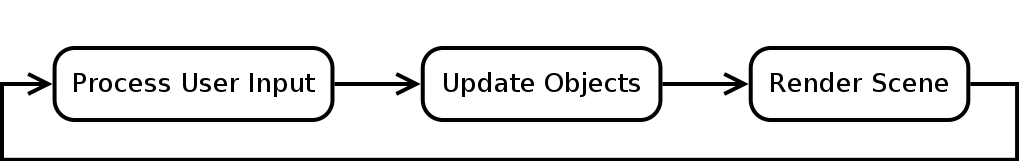
\includegraphics[width=9.25cm]{images/renderloop-simple.png}
		\caption{The most simple render loop}
		\label{fig:RenderLoopSimple}
	\end{figure}

	The disadvantage of this simple design is its dynamic frame rate -- some operations will take longer than others, resulting in greatly varying intervals between single frames, which will result in different results on different hardware. Synchronizing the output of the renderer to a fixed interval is achieved by a simple blocking operation at the end of each cycle as seen in Figure \ref{fig:RenderLoopSimpleSync}. This will guarantee an output at a fixed rate, like 30 frames/second, and allows the developer to use constant values during updates as with the previous model.

	\begin{figure}[htbp]
		\centering
		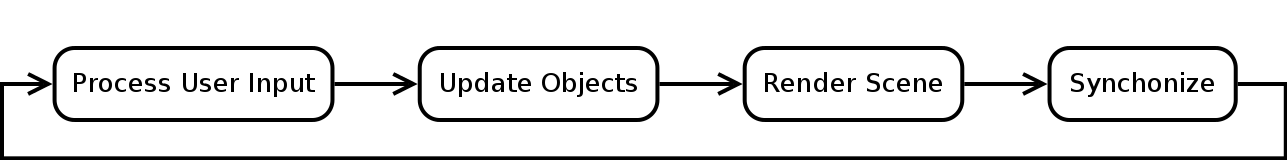
\includegraphics[width=12cm]{images/renderloop-simplesync.png}
		\caption{A simple render loop with synchronization.}
		\label{fig:RenderLoopSimpleSync}
	\end{figure}

	This approach is still insufficient, as the application starts to stutter whenever a cycle needs more time to finish than the predefined time slot. The solution is to perform all modifications to the objects in the scene using the time elapsed since the last cycle. This is the ``Single-thread Uncoupled'' model shown in Figure \ref{fig:RenderLoopDynamic}. It is further possible to add a synchronization to the end of the loop, limiting the required operations to fixed  multiples of the constants required during the loop. If a cycle needs two time slots in the example above (i.e. more than \sfrac{1}{30}, but less than \sfrac{2}{30} seconds), the next cycle will rotate the camera by 2\degree instead of 1\degreenospace.

	\begin{figure}[htbp]
		\centering
		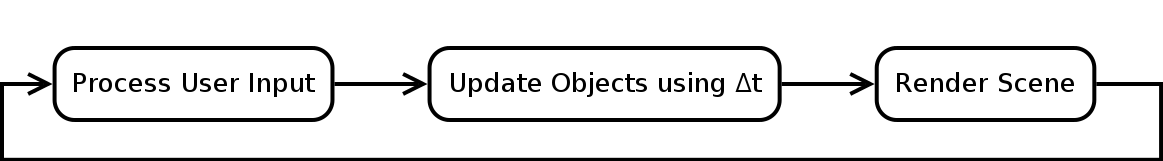
\includegraphics[width=11cm]{images/renderloop-dynamic.png}
		\caption{Single-thread Uncoupled model.}
		\label{fig:RenderLoopDynamic}
	\end{figure}

	Other models operate on multiple threads. Most importantly the rendering is performed in a separate thread, which blocks until the world updates in other threads are in a consistent state. These approaches make use of the multiple CPU cores present in today's hardware. Another big advantage of such models is that the rendering itself is performed on the GPU, while the other operations are usually bound to the CPU. All previously presented models stress either of these resources, while the other stays idle.
	
	It is possible to tackle this issue without the need for threading when using double buffering -- a common feature of modern 3d graphics cards. Most calls to OpenGL will return immediately while processing the issued command on the GPU. The call to the OpenGL function \inlinecode{SwapBuffers()} -- which flushes the rendered image onto the screen -- will block until all pending operations are finished. This makes it possible to perform other operations during this time frame. This approach is outlined in Figure \ref{fig:RenderLoopOpenGL}.

	\begin{figure}[htbp]
		\centering
		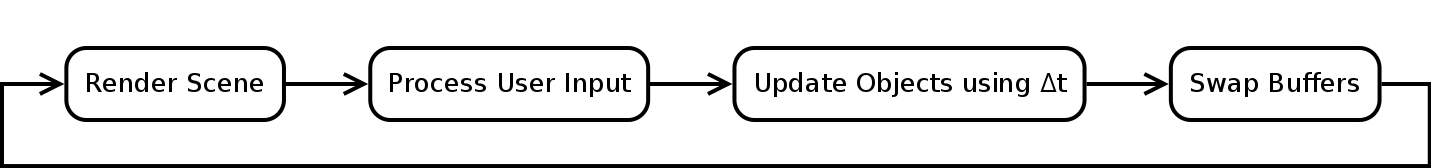
\includegraphics[width=13.5cm]{images/renderloop-opengl.png}
		\caption{A render loop in OpenGL performing operations in parallel on the CPU and the GPU.}
		\label{fig:RenderLoopOpenGL}
	\end{figure}

\section{Models}

	A \termdef{model} is a 3D object that can be positioned in space. Usually models have a predefined shape, a \termdef{mesh}, consisting of a collection of triangle definitions. The mesh alone is not enough to render any realistic scene, additional \termdef{material} definitions are attached to triangle groups which define how the triangles are to be drawn by the renderer. These materials are implemented by dedicated code fragments that run on the GPU. These self-contained applications -- so-called \termdef{shaders} -- are categorized by the objects they operate on\cite{bauchinger-2007-mre}.

	\begin{smalllist}
		\item \termdef{Vertex Shader}s operate on single vertices -- the points in the 3D-space of the mesh forming the triangles -- of the mesh. This shader type receives a single point as input and must operate on that vertex alone without any knowledge of its surroundings.
		\item \termdef{Geometry Shader}s receive multiple vertices that were processed by the vertex shaders. They have the ability to add new vertices or remove/modify existing vertices.
		\item \termdef{Pixel Shader}s (also called \termdef{Fragment Shader}s) operate on the pixels of the final image, just before it is drawn onto the screen. Figure \ref{fig:Shaders} displays a few examples of pixel shaders.
	\end{smalllist}

	\begin{figure}[htbp]
		\centering
		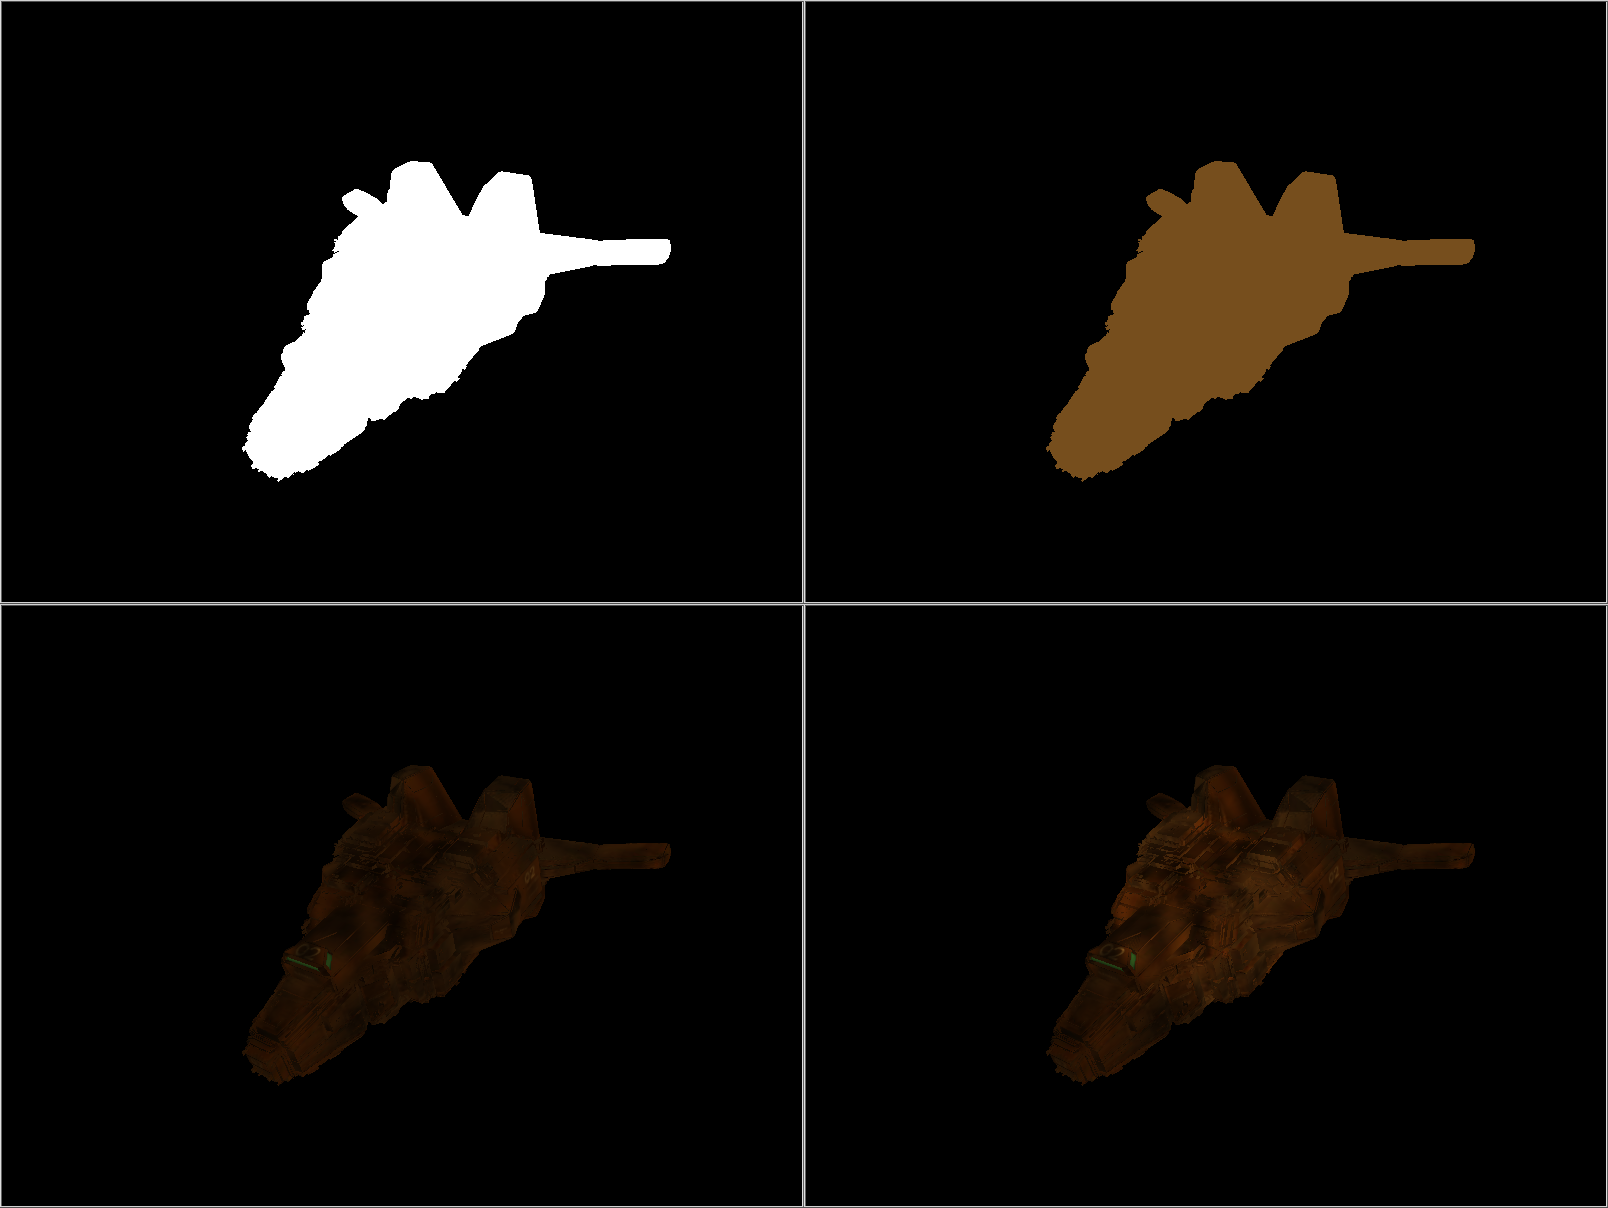
\includegraphics[width=13.5cm]{images/shaders/shaders.png}
		\caption{Examples of pixel shaders: the same model a.) without any shaders, b.) with a uniform color, c.) with a texture and d.) a shader rendering a spotlight onto it.}
		\label{fig:Shaders}
	\end{figure}

	As all of these shaders operate on tiny fragments of the complete scene, the application of the shaders can be run in parallel. Modern graphics cards can run hundreds of operations in parallel for this purpose\cite{Nvi09}.

\section{Lighting}

	Although lights are usually defined as self-contained entities in a scene, they are never drawn directly. Instead, they define how other objects in the scene are rendered. Heidrich et. al. summarize various lighting models in virtual environments in \cite{Heidrich:1999:RHS:311535.311554}. A light source usually consists of two components: diffuse and specular.

	\begin{smalllist}
		\item The diffuse component of a light ray is scattered at many angles upon hitting a surface and can thus be seen from various angles, whereas
		\item the specular component is reflected at the same angle at which it hits a surface.
	\end{smalllist}

	As light sources are only observable by the illumination of the objects in the scene, these two components are defined on the material of all surfaces, too. Whenever a diffuse (or specular) light would illuminate a surface, the material of the surface defines the effect of the illumination. A mirror will almost ignore the diffuse component of the light, but reflect the specular component with the same intensity as the incoming light beam. Most natural fabrics will do the exact opposite.

	Another property of lights is the direction the light beams are emitted towards. The common categories defined by this behavior are:

	\begin{smalllist}
		\item \termdef{point light}s -- unidirectional light sources,
		\item \termdef{spot light}s -- emitting light in a cone,
		\item \termdef{directional light}s -- coming from an infinitely distant point, giving off parallel rays -- and
		\item a single \termdef{ambient light} -- uniformly illuminating everything equally from all directions.
	\end{smalllist}

	The last parameter for light sources is their attenuation behavior -- how the light emitted from a light source is reduced depending on the distance to the surface it illuminates. This is actually rather a property of the environment in which the light source operates, as light does not fade as long as it travels unhindered in vacuum. A dusty room, on the other hand, would cause light sources to be less effective with increasing distance. The attenuation is considered a property of the light source nonetheless for technical reasons: The modification of illumination based on the properties of the sub-spaces between the surface and light source would be quite complex and computationally extremely expensive.

\section{Cameras}

	A camera is a viewpoint from which the scene is rendered. The visible space to a camera is the so-called \termdef{view frustum}\cite{Lengyel:2003:MGP:996316}, and is constrained by the near and far clip distances as seen in Figure \ref{fig:CameraFrustum}. Solely objects within -- or reaching into -- this area are rendered when viewing the scene from this camera.

	\begin{figure}[htbp]
		\centering
		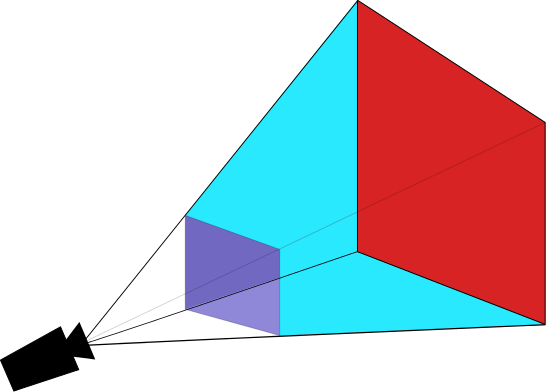
\includegraphics[width=9cm]{images/frustum.png}
		\caption{The view frustum of a camera, contained by the \emph{near clip distance} in purple and the \emph{far clip distance} in red.}
		\label{fig:CameraFrustum}
	\end{figure}

	The other two parameters for the definition of a camera are its field of view -- the horizontal angle of the frustum -- and the aspect ratio defining the vertical angle. It is possible to establish further properties that simulate the effects of different camera lenses\cite{Kolb:1995:RCM:218380.218463}, but we will limit our model to the simplified definition above.

